\documentclass[12pt,a4paper,twoside]{article}
\usepackage[english]{babel} % serve a far si che i capitoli vengano scritti in italiano
\usepackage[utf8]{inputenc} % serve per scrivere direttamente i caratteri accentati
\usepackage[T1]{fontenc} 
\usepackage{microtype} 
\usepackage{graphicx} % serve per le
\usepackage{amssymb}
\usepackage{mathrsfs}
\usepackage{framed}
\usepackage{bm}
\usepackage{fancybox}
\usepackage{textcomp} %per inserire �
\usepackage{colortbl} %serve per colorare le tabelle
\usepackage{color}
\usepackage{hyperref} %[colorlinks=false]
\usepackage{amsfonts}
\usepackage{listings} %per l'inserimento di codice
\usepackage{amsmath} %testo dentro equazioni
\usepackage{mathrsfs}
\usepackage{graphicx}
\usepackage{subcaption} %matrice di immagini
%\usepackage{subfigure}
\usepackage[tight,italian]{minitoc} % mini indice
\usepackage{rotating}
\usepackage{caption}
\usepackage{enumerate}
\usepackage{graphicx}
\usepackage{multimedia}
\author{Fabio Busignani}
\title{Google Glass Project}
\graphicspath{{images/}}
\begin{document}
	\maketitle
	\clearpage
	The \textit{organs-on-a chip} platforms seek to recapitulate human organ function at micro-scale by integrating microfluidic networks with three-dimensional organ models, which are expected to provide robust and accurate predictions of drug/toxin effects in human bodies. In fulfilling this aim, a set of physical/chemical parameters need to be monitored and stored in order to capture such effects of drug/toxin administered into the system.\\
	Such kind of monitoring and storing process has been designed using the Google Glass platform as illustrated in (Fig.\ref{Fig:BlockDiagram}).
	
	\begin{figure}[h]
		\centering
		\includegraphics[width = \textwidth]{Intro/Block_Diagram.eps}
		\caption{Block diagram of the system}
		\label{Fig:BlockDiagram}
		
	\end{figure}
	
	The (Fig.\ref{Fig:BlockDiagram}) shows the principal steps of data transmission from physical and video sensors to the Google Glass via an \textit{Embedded Linux System} performed using the \href{http://beagleboard.org/BLACK}{\textbf{Beaglebone Black}}.\\
	The Beaglebone Black runs processes that are in charged to:
	\begin{itemize}
		\item acquire the sensors value and to store them onto \textit{Google App Engine Data Storage};
		\item acquire the video, perform the beating plot, and to store them onto \textit{Google App Engine Data Storage};
		\item get from the \textit{Google App Engine Data Storage} the electrovalves status set from the user through the Google Glass and to drive the electrovalves.
	\end{itemize} 
	
	The whole designed environment includes a program, written using the framework \textit{Qt}, for storing the recorded video from microscope.
	
	\section*{Preview of the Glasswear}
	\addcontentsline{toc}{section}{Preview of the Glasswear}
	The (Fig.\ref{Fig:GlasswearDiagram}) shows the structure of the Glasswear. From the Home Screen (Fig.\ref{Fig:GlasswearDiagram}a), using the voice trigger "\textit{Show Measurement}" or tapping on the "\textit{Measurement}" card (Fig.\ref{Fig:GlasswearDiagram}b) user is allowed to enter in the application (Fig.\ref{Fig:GlasswearDiagram}c). From this point, tapping and swiping, it's possible to navigate into the glasswear's menu (Fig.\ref{Fig:GlasswearDiagram}d-h) and choose which card has to be shown. \textit{View PH} (Fig.\ref{Fig:GlasswearDiagram}i) and \textit{View Temperature} (Fig.\ref{Fig:GlasswearDiagram}j) cards  plot on the card's left side the value of pH and temperature, respectively. While on the right side they show the average value. The microscope's video is shown by tapping on \textit{View Video} (Fig.\ref{Fig:GlasswearDiagram}k). The \textit{View Beating} card (Fig.\ref{Fig:GlasswearDiagram}l) shows the graph of the beating associated to the video.
	\\
	
	\begin{figure}[h]
		\centering
		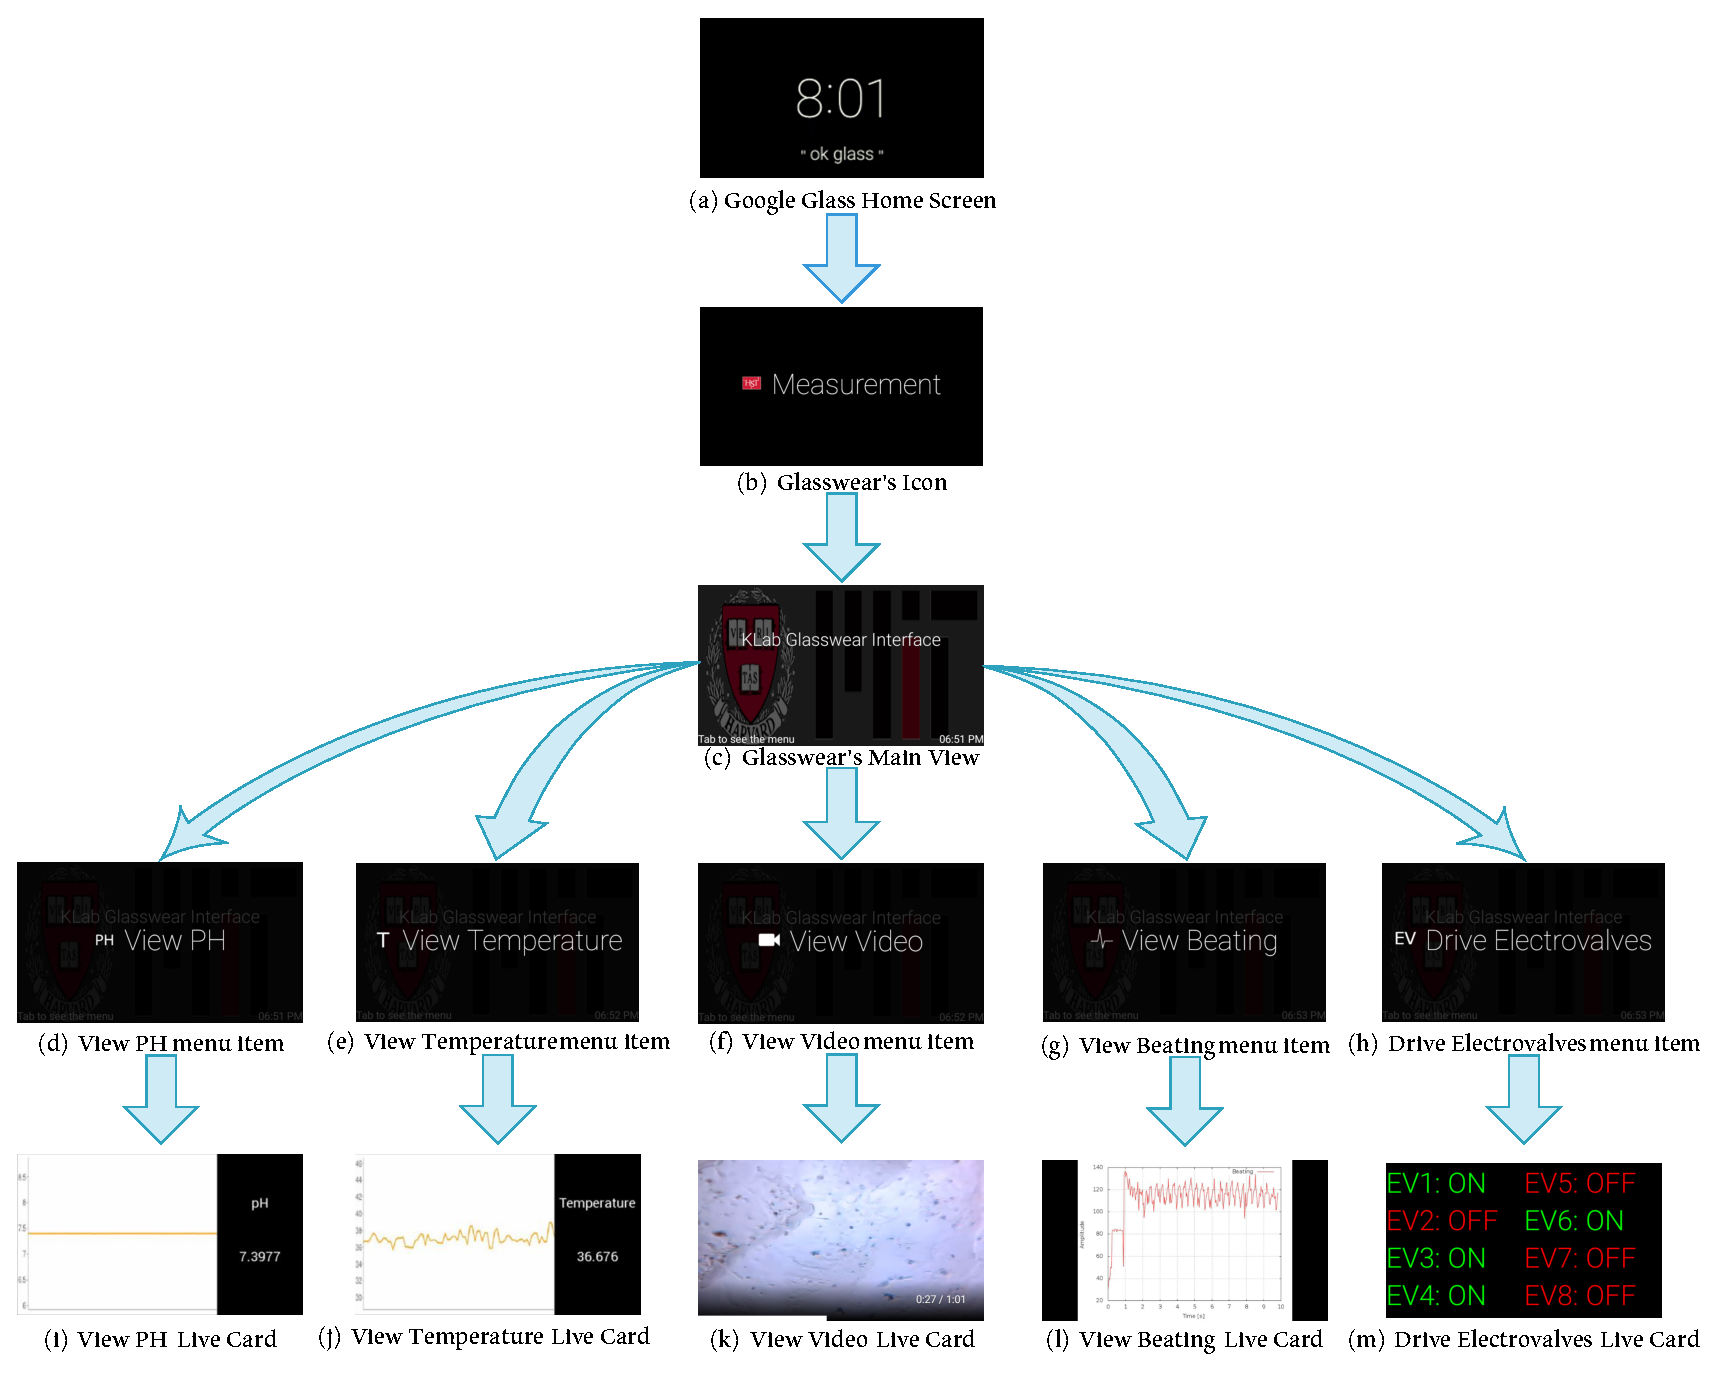
\includegraphics[width=\textwidth]{Intro/block-app.eps}
		\caption{Glasswear's Block Diagram}
		\label{Fig:GlasswearDiagram}
	\end{figure}
	
	
	From the \textit{Drive Electrovalves} card (Fig.\ref{Fig:GlasswearDiagram}m), the user can set the value of each electrovalve. The main view of this card shows the status of each electrovalve (written in green if it is on and in red if it is off).
	\clearpage
	\begin{figure}[h]
		\centering
		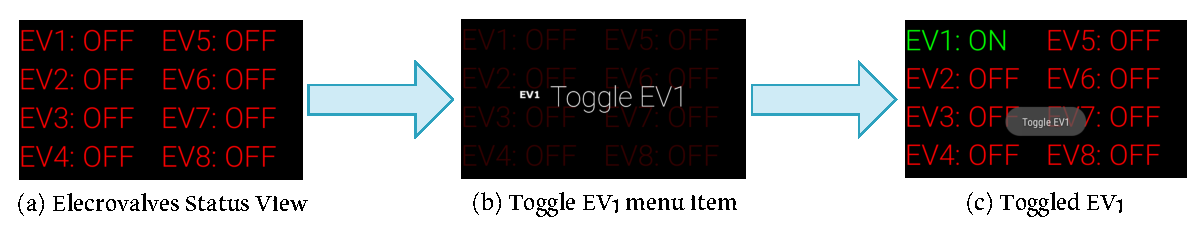
\includegraphics[width=\textwidth]{Intro/electrovalves.eps}
		\caption{Drive Electrovalves Steps}
		\label{Fig:Electrovalves}
	\end{figure}
	
	The (Fig.\ref{Fig:Electrovalves}) shows the steps to toggle the status of the first electrovalve:
	\begin{enumerate}
		\item (Fig.\ref{Fig:Electrovalves}a) shows the initial status of the whole electrovalves (all off);
		\item tapping on the card and swiping the user is allowed to change the status of each electrovalve from the menu, as shown in (Fig.\ref{Fig:Electrovalves}b);
		\item after that the electrovalve has been chosen, a toast message pops up (Fig.\ref{Fig:Electrovalves}c), and the new values of the electrovalves are shown. 
	\end{enumerate}
	
	To return on the main card of the glassware, the user has to tab on \textit{Back} item (Fig.\ref{Fig:Back}) from every menu.
	
	\begin{figure}[h]
		\centering
		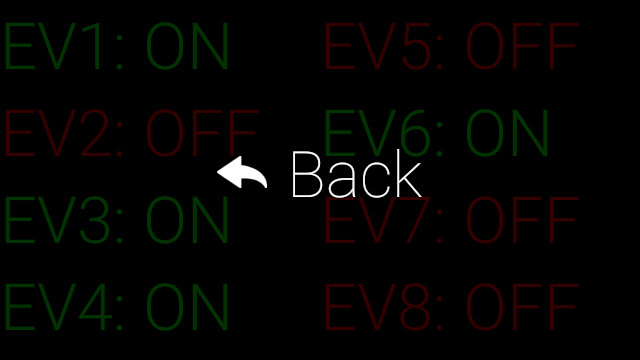
\includegraphics[scale=.28]{Intro/back_menu}
		\caption{\textit{Back} menu item}
		\label{Fig:Back}
	\end{figure}
	
	To terminate the glassware, from every menu, the user has to swipe up to the final item and tab on \textit{Exit} item (Fig.\ref{Fig:Exit}).
	
	\begin{figure}[h]
		\centering
		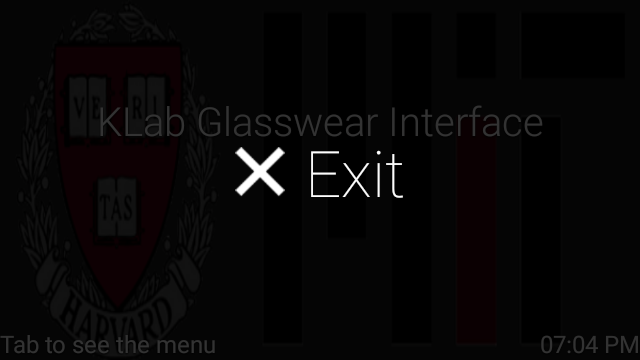
\includegraphics[scale=.28]{Intro/exit}
		\caption{\textit{Exit} menu item}
		\label{Fig:Exit}
	\end{figure}
	
	\section*{Experiments With Driver for Electrovalves}
	
	In order to try the reverse control from the Google Glass to the electrovalves we made different kind of experiments.\\
	
	\subsection*{LED Experiments}
	 First of all we tried the circuit on a breadboard using LEDs instead of electrovalves. The aim of this step is to demonstrate that the firmware running on the Beaglebone Black, the Java code running on the Google Glass and the Python code running on the Google App Engine (used to store the information about the electrovalves status) work well.\\
	Moreover the LED and the electrovalve have basically the same behavior so, if everything works well with the LEDs, there are all the reasons to believe that everything is going to work well with the electrovalves, too.\\
	
	The circuit that actually drives the LEDs is very simple, and it is based on a MOS transistor (\href{http://www.onsemi.com/pub_link/Collateral/BS170-D.PDF}{\textit{BS170}}) used as a switch voltage-controlled, as shown in (Fig.\ref{Fig:driverLED}).
	
	\begin{figure}[h]
		\centering
		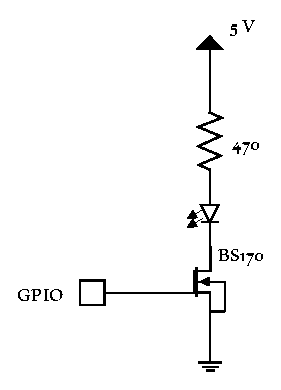
\includegraphics[]{Driver/driverLED}
		\caption{Driver for LED}
		\label{Fig:driverLED}
	\end{figure}
	
	The (Fig.\ref{Fig:circuitLED}) shows the circuit used for this step of testing. As can be seen the number of LEDs used is eight, the same number of electrovalves that can be driven from this system.\\
	In order to test all of them we made 2 different kind of trials:
	\begin{enumerate}
		\item \textit{In order turning on\&off}, first all the LEDs are turned on starting from the first one (on the top right corner) to the last one (on the bottom left corner). Then the LEDs are turned off following the same order.\\The result of this can bee watched in  \href{http://youtu.be/iYeAMpxM9uI}{\textbf{this}} video.
		\item \textit{Out of order turning on\&off}, in this trial, like before, all the LEDs start from a condition where all of them are off and then we turned on and off all the LEDs, but in this case following a random order.\\ The result of this can bee watched in  \href{http://youtu.be/mIoylW334Ck}{\textbf{this}} video.
	\end{enumerate}
	
	
	\begin{figure}[h]
		\centering
		\includegraphics[scale=.21]{Experiments/ledBoard}
		\caption{LEDs experiments board}
		\label{Fig:circuitLED}
	\end{figure}
	
	
	\subsection*{Electrovalves experiments}
	
	\subsubsection*{Breadboard Phase}
	The (Fig.\ref{Fig:circuitBreadboard}) shows from the top view the circuit used during the second phase of experiment, the one where we started using electrovalves in a real microfluidic application.\\
	On the left side of the figure we can see the conditioning circuits for the temperature sensor (on the top) and pH sensor (on the bottom). While, on the other side, we can see the part of circuit in charge to drive the electrovalves.\\
	In this last one we are going to focus for now. Each electrovalve is driven by the circuit shown in (Fig.\ref{Fig:driverEV}).
	\clearpage
	
	\begin{figure}[h]
		\centering
		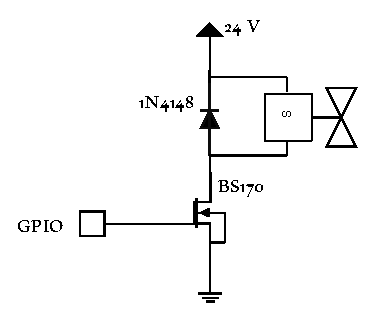
\includegraphics[]{Driver/driverEV}
		\caption{Driver for electrovalves}
		\label{Fig:driverEV}
	\end{figure}
	
	As you can see, this circuit is pretty close to the one of (Fig.\ref{Fig:driverLED}), indeed the only difference is given by freewheeling diode, mandatory because of inductive behavior of electrovalve's solenoid.
	
	\begin{figure}[h]
		\centering
		\includegraphics[scale=.14]{circuitBreadboard}
		\caption{Circuit mounted on breadboard top view}
		\label{Fig:circuitBreadboard}
	\end{figure}
	
	
	The result of the experiments with electrovalves in a real microfluidic case can bee watched in  \href{https://www.youtube.com/watch?v=CavCVnD2P1k}{\textbf{this}} video.
	
	\begin{figure}[h]
		\begin{center}
		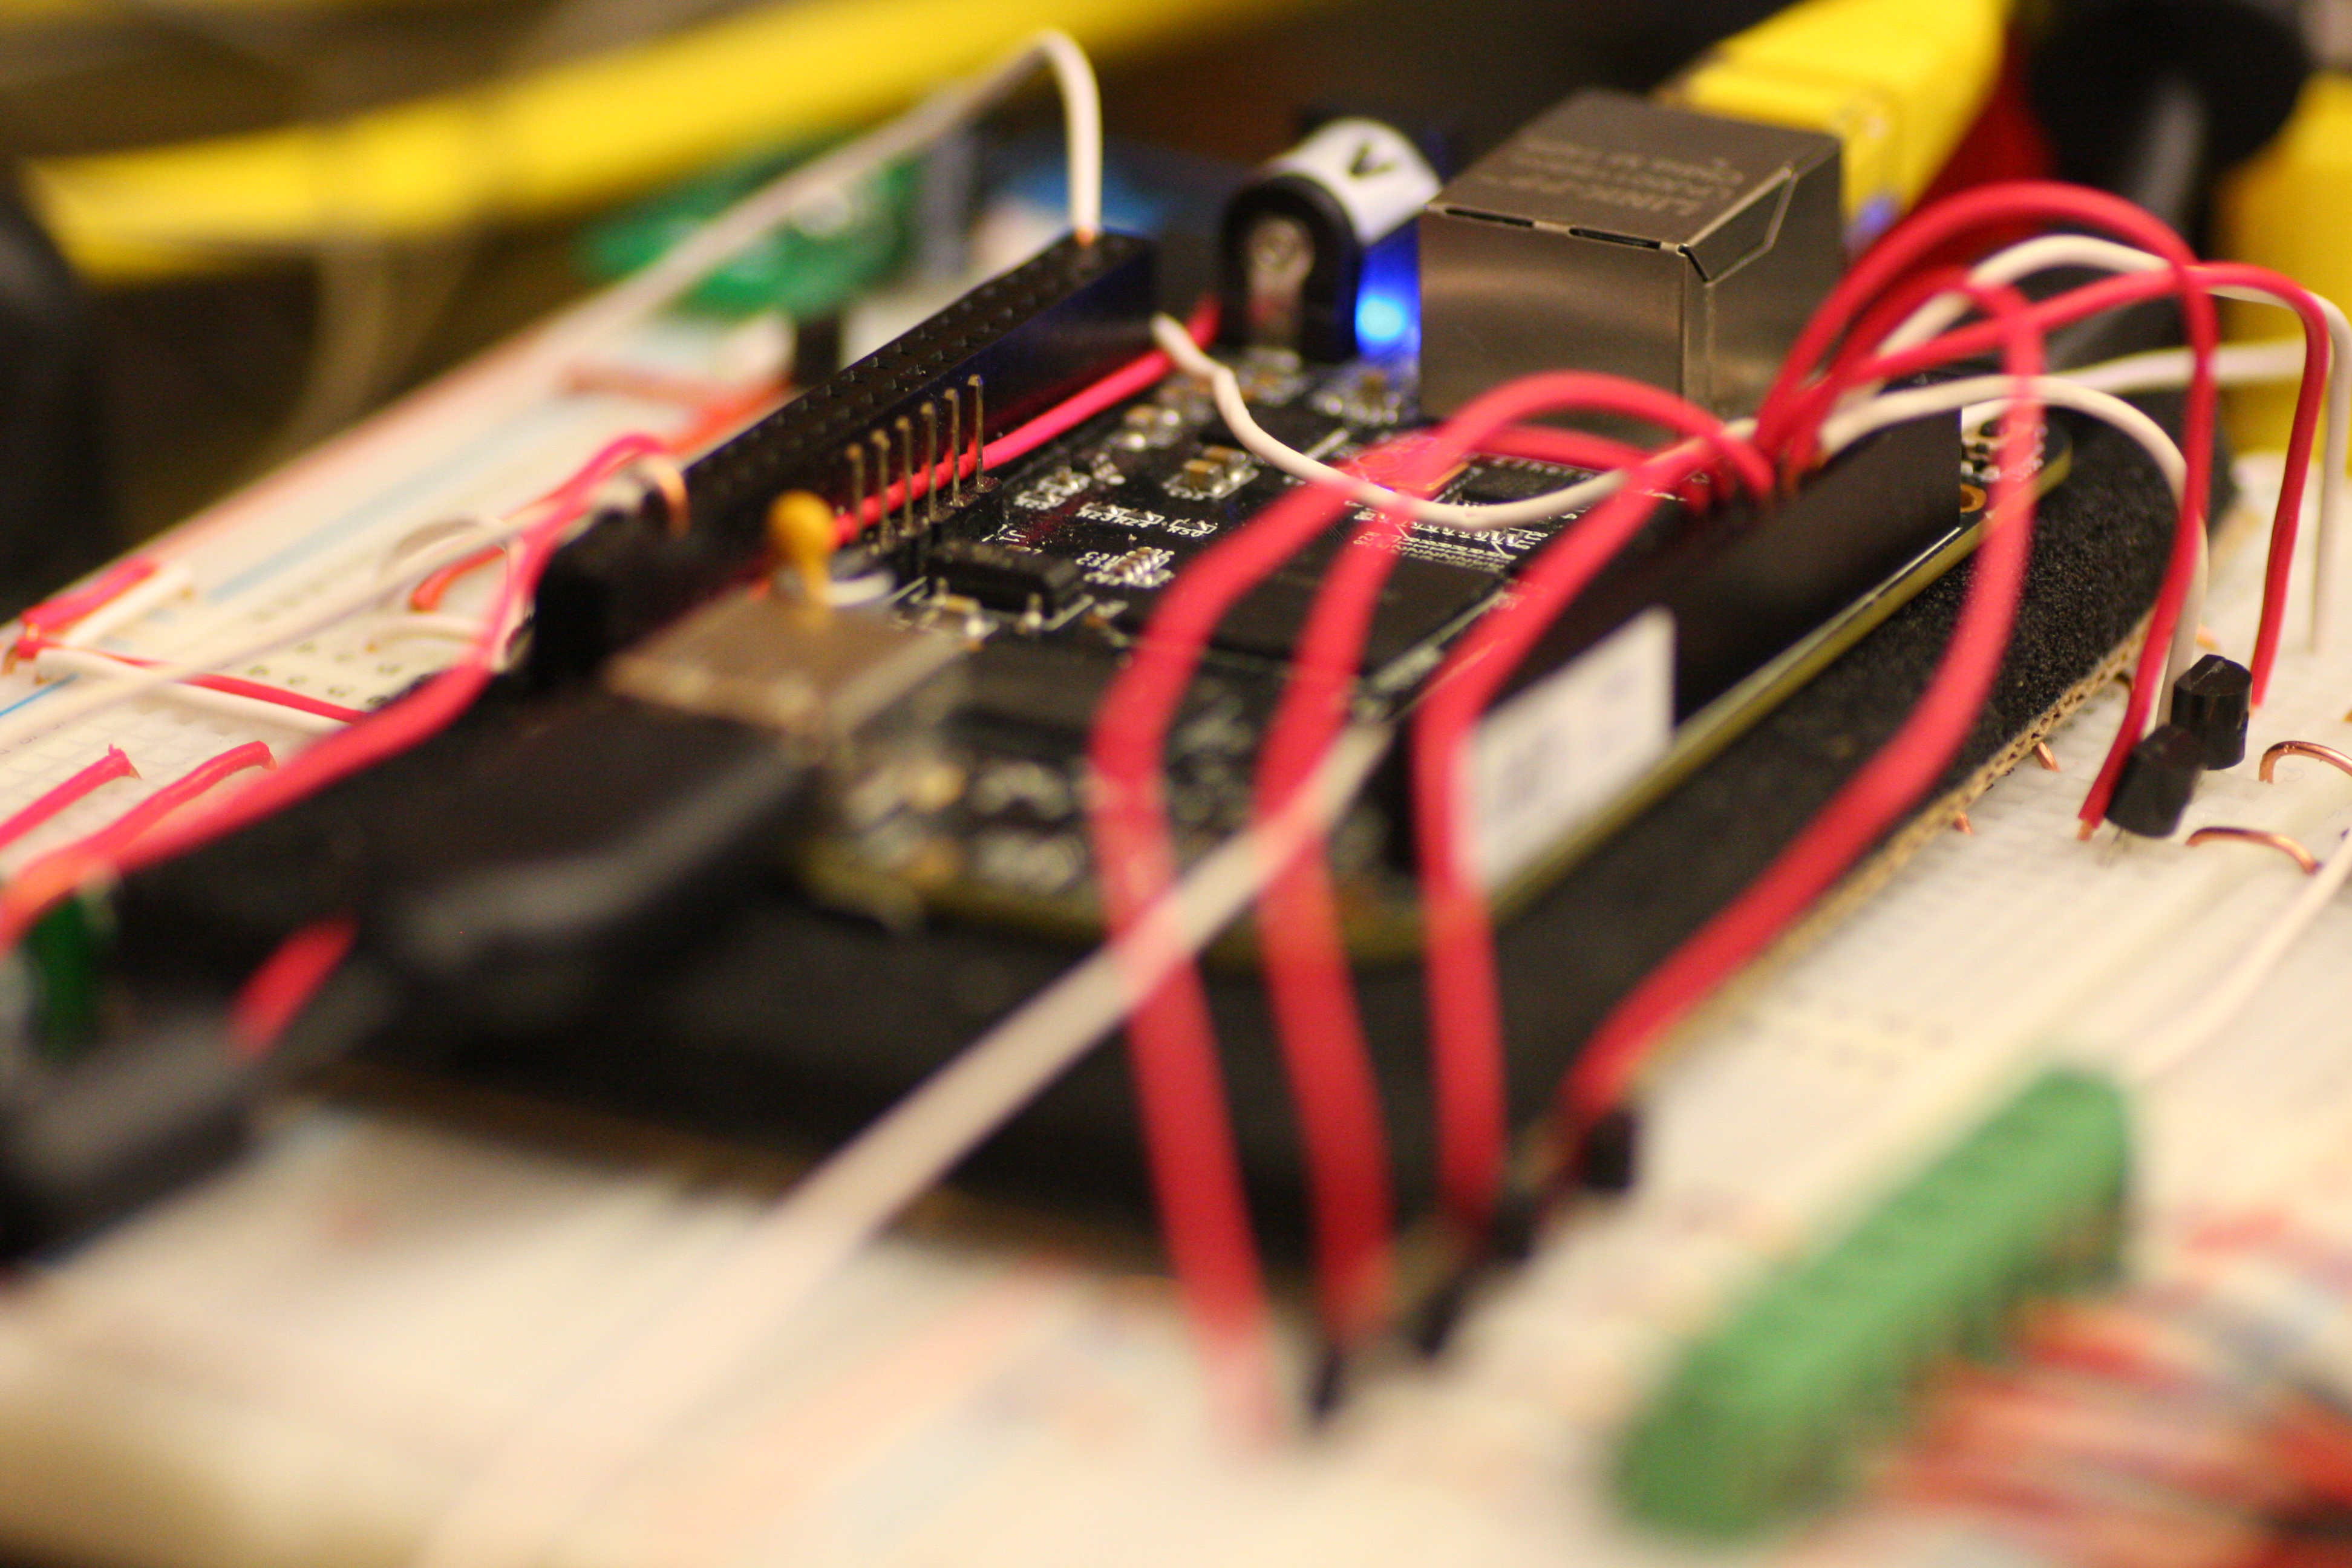
\includegraphics[width=\textwidth]{breadboard}
		\caption{Circuit mounted on breadboard side view}
		\label{Fig:circuitsfumatp}
	\end{center}
	\subsubsection*{PCB Phase}
	
	Finally we replied the last experiment using a PCB (Fig.\ref{fig:PCB}),  designed for this system.\\
	In (Fig.\ref{fig:3dmodel}) the 3D model made during the project phase is shown, while (Fig.\ref{fig:tiger}) shows its real realization.\\
	As expected the result of this experiment is the same of the previus step. 
	\end{figure}
	
	
	
	
	\begin{figure}
		\centering
		\begin{subfigure}[h]{0.5\textwidth}
			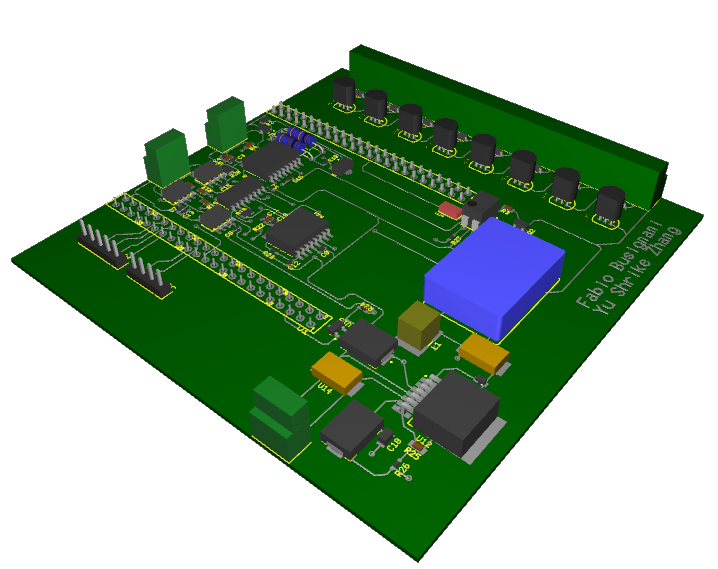
\includegraphics[width=\textwidth]{pcb/3D-circuit-green}
			\caption{PCB 3D Model}
			\label{fig:3dmodel}
		\end{subfigure}%
	~
		\begin{subfigure}[h]{0.5\textwidth}
			\includegraphics[width=\textwidth]{pcb/foto}
			\caption{PCB Real Result}
			\label{fig:tiger}
		\end{subfigure}
			\caption{System's PCB}\label{fig:PCB}
	\end{figure}
	
	\begin{figure}[h]
		\centering
		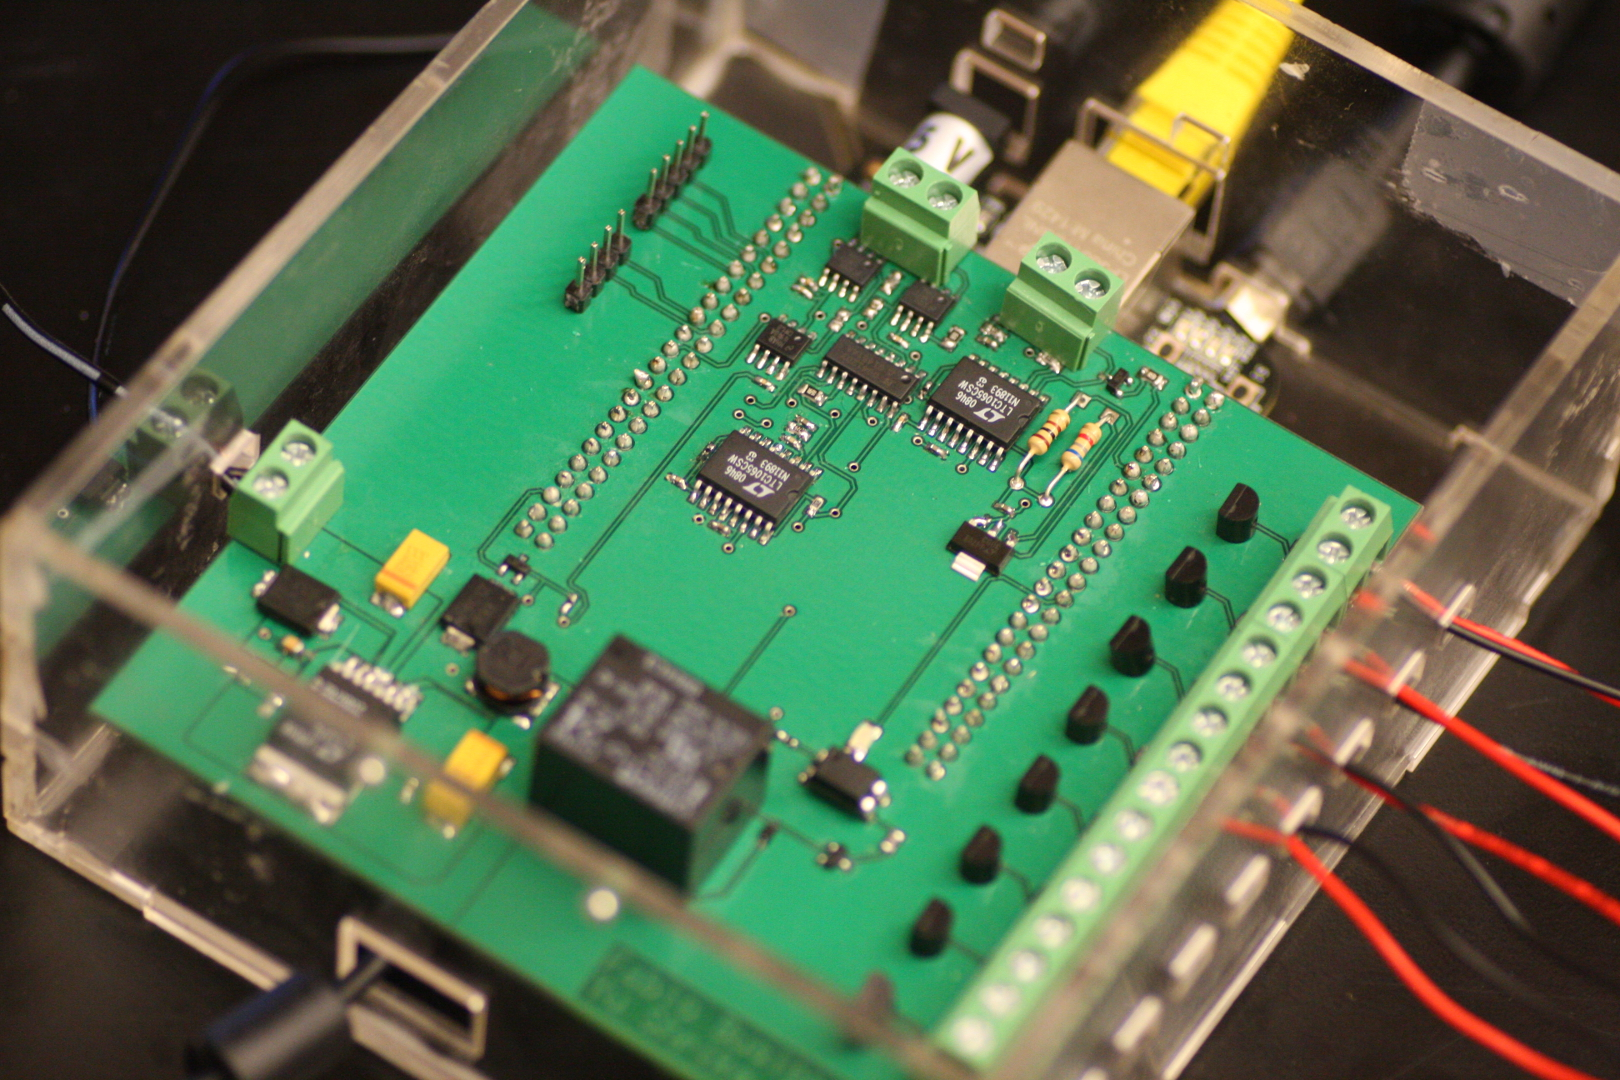
\includegraphics[width = \textwidth]{circuitfinisched}
		\caption{Final system mounted on a PCB}
		\label{Fig:finalcircuit}
	\end{figure}
	\clearpage
	\section*{Store Microscope Video}
	The storing of the microscope video plays an important role of this system. It may be essential to review the recorded video  during the experiment and in order to fulfill this aim a \textit{Qt} program has been designed.\\
	We chose \textit{Qt} because in this way the program is available for different operating systems, \textit{Linux}, \textit{Windows}, and \textit{MacOS}.\\
	
	The program is very easy to use, the user just has to run the executable (Fig.\ref{Fig:icostoring}).
	
	\begin{figure}[h]
		\begin{center}
			\includegraphics[scale=.5]{storing/Icon}
			\caption{Storing Microscope Video Program's Icon}
			\label{Fig:icostoring}
		\end{center}
	\end{figure}
	
	Once it has been launched, a console is opened (Fig.\ref{Fig:storingwindows}). The program checks every 20 seconds if a new video has been uploaded on the server. If so, the new video will be stored inside the computer (directory \texttt{C:/Video}) with the current data and hour as name in the following form: $YYYY-MM-DD-HH-mmss$.\\
	
	As shown in (Fig.\ref{Fig:storingwindows}) on the console the user can read all the information about what the program is doing.
	
	\begin{figure}[h]
		\begin{center}
			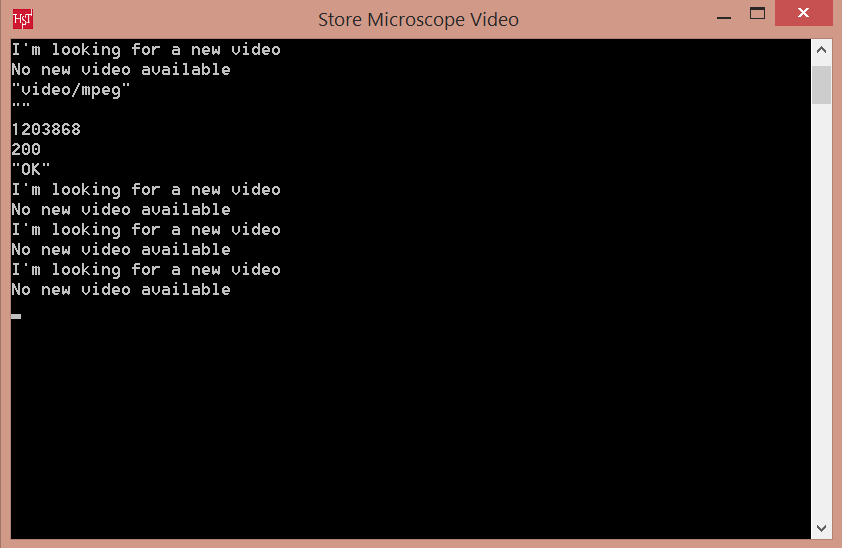
\includegraphics[scale=.7]{storing/program-windows}
			\caption{Storing Microscope Video Console}
			\label{Fig:storingwindows}
		\end{center}
	\end{figure}
	
\end{document}